
\documentclass[UTF8,a4paper,12pt]{ctexart}
\usepackage{geometry}
\geometry{top=2.54cm,bottom=2.54cm,left=3.17cm,right=3.17cm}
\usepackage{amsmath,amssymb,booktabs,array,graphicx,float,setspace,caption,hyperref,threeparttable,longtable}
\hypersetup{colorlinks=true,linkcolor=black,urlcolor=black,citecolor=black}
\setstretch{1.35}
\ctexset{
  section={format=\heiti\zihao{3}, name={,}, number=\arabic{section}.},
  subsection={format=\heiti\zihao{4}, name={,}, number=\arabic{section}.\arabic{subsection}}
}
\captionsetup{font=small,labelfont=bf,labelsep=quad}
\graphicspath{{../benchmark/}{./}}
\pagestyle{plain}
\begin{document}
\begin{titlepage}
\thispagestyle{empty}
\centering
\vspace*{1.35cm}

\includegraphics[width=6.0cm]{guangzhou_university.png}\par
\vspace{1.45cm}
{\heiti\zihao{1} 《回归分析》课堂论文\par}
\vspace{3.25cm}
\renewcommand{\arraystretch}{1.45}
\begin{tabular}{>{\centering\arraybackslash\heiti\zihao{4}}p{3.0cm}@{\hspace{0.4cm}}>{\zihao{4}\arraybackslash}p{9.2cm}}
论文题目 & 基于新浪财经数据的 A 股指数增强模型收益回归分析 \\
\cline{2-2}
学\quad 院 & 数学与信息科学学院 \\
\cline{2-2}
专\quad 业 & 数学与应用数学 \\
\cline{2-2}
学生姓名 & 吴泽 \\
\cline{2-2}
学\quad 号 & 32315100009 \\
\cline{2-2}
\end{tabular}
\end{titlepage}

\begin{center}
{\heiti\zihao{3} 基于新浪财经数据的 A 股指数增强模型收益回归分析}
\end{center}

\noindent\textbf{摘要：}本文以一个完整可复现的A股量化项目为研究对象，使用新浪财经公开接口获取股票列表、股票日K线、复权因子和指数行情数据，经过清洗后转换为Qlib可用格式，并在Qlib框架下运行Alpha158-LightGBM模型形成样本外选股信号。与一般量化项目报告不同，本文严格按照回归分析课程论文的要求，将策略回测结果转化为可检验的计量问题：以策略测试期日收益率为被解释变量，以上证指数收益率、深证成指收益率、中证500收益率、换手率和交易成本率为解释变量，建立多元线性回归模型，分析策略收益与市场风险暴露、交易行为变量之间的关系。本文进一步进行描述性统计、相关性分析、多重共线性检验、异方差检验、自相关检验、残差正态性检验和稳健性讨论。研究发现，在“上一交易日收盘后生成信号、下一交易日开盘成交”的较保守设定下，策略样本外收益仍高于主要市场基准；但回归结果显示，策略收益并非完全独立于市场行情，而是显著暴露于上证指数和中证500等市场变量。本文认为，该项目适合作为回归分析方法在金融数据中的应用案例，其回测收益应被理解为研究性结果，而不能直接等同于实盘可得收益。

\noindent\textbf{关键词：}回归分析；A股量化；多元线性回归；稳健标准误；Qlib；LightGBM；市场暴露

\section{前言}
金融市场研究中的一个重要问题是：某一投资策略获得的收益究竟来自真实的选股能力，还是来自市场整体上涨、行业风格暴露、交易规则假设或样本选择偏差。对于传统资产定价研究而言，这一问题通常通过回归分析解决。例如，将股票或投资组合收益率作为被解释变量，将市场收益率、规模因子、价值因子、动量因子等作为解释变量，通过回归系数判断收益来源和风险暴露。早期CAPM模型强调市场风险对资产收益的解释作用\cite{sharpe1964}，后续多因子模型则进一步把规模、价值、动量等因素纳入收益解释框架\cite{fama1993,jegadeesh1993,carhart1997}。对于机器学习量化策略而言，虽然模型结构更加复杂，预测变量也更加高维，但策略最终呈现出来的仍然是一条日频收益序列，因此同样可以通过回归模型解释其收益来源。

本文的研究背景来自一个已经搭建完成的A股量化项目。为保证课程作业的可复现性和提交材料的完整性，项目代码、配置文件、结果摘要、论文TeX源文件和最终PDF已经上传至GitHub仓库：\url{https://github.com/skdhod/Regression_analysis}。仓库中不直接提交大体量原始行情数据和Qlib二进制数据，而是保留可复现脚本，使读者能够按照相同流程重新抓取和生成数据。该项目不使用商业数据源，而是直接使用新浪财经公开接口抓取数据：一方面抓取A股股票列表、股票日K线和复权因子；另一方面抓取上证指数、深证成指、上证100、深证100和中证500等基准指数。数据经过标准化清洗后转换为Qlib格式，再使用Alpha158特征和LightGBM模型进行训练、预测和回测。项目工程链条本身较长，包含接口探测、数据抓取、复权处理、Qlib格式转换、模型训练、策略回测和结果分析等环节。但如果仅停留在工程实现和净值展示层面，就不符合回归分析课程的核心要求。因此，本文将该项目进一步转化为回归分析问题：在测试期内，策略每日收益率是否能够被主要市场指数收益解释？换手率和交易成本是否与策略收益存在统计关系？模型残差是否满足经典线性回归的基本假设？

本文的研究意义主要体现在三方面。第一，从方法角度看，本文展示了如何把机器学习量化回测结果转化为回归分析对象，使“黑箱式”的选股模型结果能够被传统计量方法解释。第二，从实证角度看，本文通过多个市场基准变量检验策略收益的市场暴露，避免只凭策略净值曲线得出过度乐观结论。第三，从课程训练角度看，本文完整呈现了变量选取、模型设定、参数估计、显著性检验和诊断检验，能够体现回归分析课程中关于多元线性回归、异方差、共线性和残差诊断等知识点的综合运用。

需要说明的是，本文并不试图证明该量化策略已经达到实盘交易标准。相反，本文在论文中主动讨论该项目的局限性，包括当前时点股票池可能带来的幸存者偏差、公开接口数据并非严格point-in-time数据库、真实交易中可能存在更高滑点和冲击成本等。这些限制并不会削弱本文作为回归分析课程论文的价值，因为课程论文的重点并不是宣传策略收益，而是说明如何利用回归工具识别和解释策略收益。

从回归分析课程的角度看，本文的核心并不是“预测股票涨跌”，而是围绕一个可观察的因变量建立解释框架。量化项目输出的预测分数、持仓变化和组合净值，本身只是原始研究材料；只有把这些材料整理成被解释变量、解释变量和控制变量，再给出模型形式、估计方法、检验方法和经济解释，才构成一篇规范的实证论文。因此，本文在写作上有意弱化模型工程细节，强化变量关系和统计检验：先说明为什么要把策略收益放在市场收益背景下考察，再说明为什么需要控制换手率和成本率，最后通过回归结果讨论策略收益中哪些部分可以被市场解释，哪些部分可能属于模型带来的剩余收益。这样的研究思路与课程中“用回归模型解释现实经济问题”的训练目标是一致的。

\begin{figure}[p]
\centering
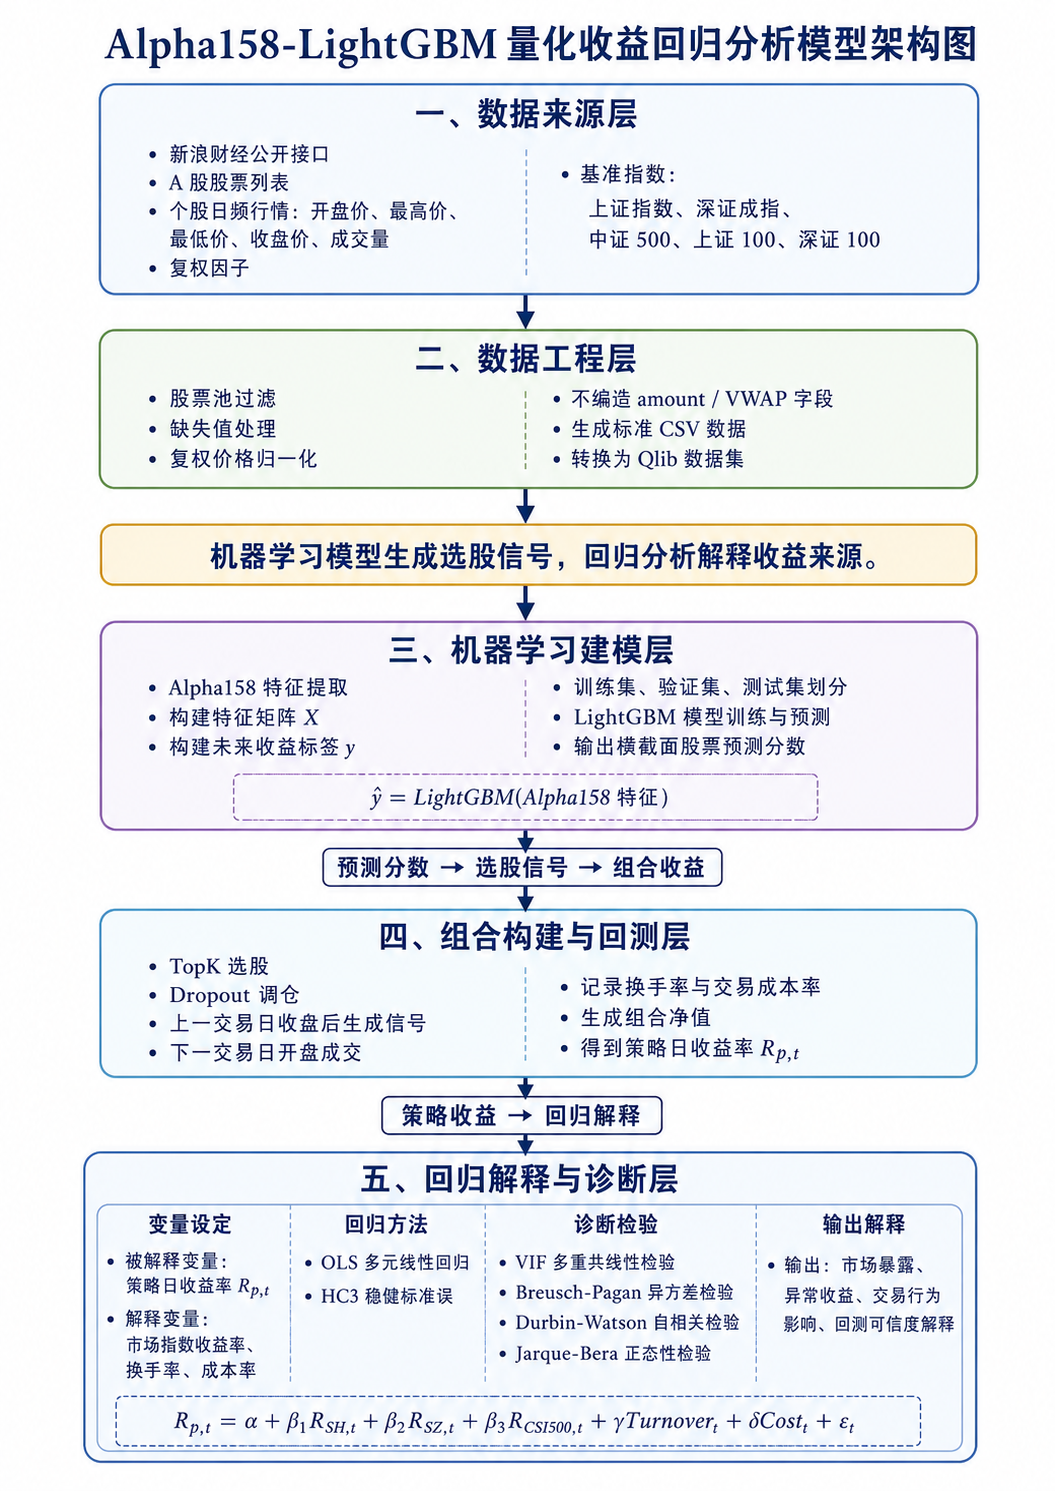
\includegraphics[height=0.84\textheight]{paper_flow_external.png}
\caption{项目数据处理与回归分析流程}
\label{fig:flow}
\end{figure}

\section{国内外研究现状}
\subsection{资产收益解释模型}
资产收益的回归解释是金融计量研究中的经典主题。资本资产定价模型将单个资产或投资组合的超额收益表示为市场超额收益的线性函数，其中市场beta用于衡量资产对市场系统性风险的暴露\cite{sharpe1964}。该模型虽然形式简单，但提供了一个非常重要的研究思路：投资收益不能只看绝对大小，还要看其承担了多少系统性风险。若一个策略收益很高，但其beta也很高，那么收益很可能主要来自市场上涨；若控制市场收益后常数项仍显著为正，则可以进一步讨论其异常收益。

Fama和French在此基础上提出三因子模型，将规模和价值因子纳入回归框架，说明股票收益不仅受市场风险影响，还受公司规模和账面市值比等风格因子的影响\cite{fama1993}；其五因子模型又进一步加入盈利能力和投资风格变量\cite{fama2015}。Jegadeesh和Titman关于动量收益的研究以及Carhart四因子模型也表明，价格趋势变量可以成为收益解释的重要组成部分\cite{jegadeesh1993,carhart1997}。虽然这些模型在因子选择上有所不同，但共同点是使用线性回归估计风险暴露，通过显著性检验判断某一变量是否对收益具有解释力。本文虽然没有完整构造Fama-French因子，但采用上证指数、深证成指和中证500作为市场与板块代理变量，本质上仍属于收益归因型回归分析。

\subsection{机器学习与量化选股}
随着数据规模扩大和计算能力提升，机器学习方法越来越多地应用于量化投资。传统线性模型通常要求研究者事先设定变量关系，而机器学习模型能够从大量特征中学习非线性关系和交互效应。Gu、Kelly和Xiu的研究说明，机器学习方法能够在大规模资产定价数据中捕捉非线性预测信息\cite{gu2020}。LightGBM作为梯度提升树模型，具有训练速度快、处理非线性能力强、适合表格数据等优点，因此常用于股票横截面排序任务\cite{ke2017}。Qlib平台则提供了标准化的数据管理、特征表达、模型训练和回测接口，适合构建可复现的量化研究流程\cite{yang2020,qlibgithub}。

但是，机器学习模型在金融场景中也更容易出现研究偏误。一方面，金融数据具有低信噪比、非平稳和结构突变等特点，模型在训练期表现良好并不必然意味着样本外稳定有效。另一方面，量化回测对数据时点和交易时点极其敏感，如果使用未来数据、当前股票池回看历史、或用当天收盘后才能知道的信号按当天收盘成交，就会产生未来函数。本文在项目运行过程中曾发现，若使用较理想的收盘成交假设，策略收益显著偏高；将成交假设改为下一交易日开盘成交后，收益明显下降。这也说明，对于机器学习量化策略，回归分析和回测审计同样重要。

\subsection{回归诊断相关研究}
经典线性回归模型要求误差项满足零均值、同方差、无自相关以及解释变量不存在完全多重共线性等条件。在金融收益率数据中，这些条件往往难以完全满足。例如，市场波动具有聚集性，容易导致异方差；不同市场指数之间高度相关，容易导致共线性；策略收益可能受调仓周期和持仓延续影响，残差也可能存在自相关。因此，实证金融研究通常不会只报告普通OLS系数，而会结合稳健标准误、VIF、Breusch-Pagan检验、Durbin-Watson统计量和残差分布检验共同判断模型质量\cite{white1980,breusch1979,durbin1951,jarque1980}。

\subsection{文献评述}
综合已有文献可以看到，传统资产定价模型重视可解释性，机器学习量化模型重视预测能力，两者并不是相互排斥的。本文的处理方式是先使用机器学习模型生成策略收益，再使用回归模型解释收益来源。这样既保留了量化项目的实证背景，也使论文核心落在回归分析。本文的不足在于，受公开数据源限制，尚未构造严格的历史成分股池和完整风格因子；但作为课程论文，本文已经能够完整展示从数据构造、变量定义、模型估计到诊断解释的回归分析过程。

进一步看，国内很多量化研究报告更关注收益率、夏普比率和最大回撤，容易把回测绩效指标当作最终结论；而回归分析要求研究者追问“为什么会有这样的收益”。如果策略收益主要由市场指数解释，那么高收益可能只是承担了更高市场风险；如果在控制市场变量后仍有显著正的常数项，才有理由进一步讨论选股模型的增量贡献。本文正是在这一意义上将量化回测结果重新解释为回归问题。它不否认机器学习模型的价值，但强调任何机器学习结果都需要经过统计检验、经济解释和稳健性讨论，否则很容易形成“看起来有效、实际不可交易”的结论。

\section{指标选取和模型设定}
\subsection{指标选取}
本文以2025年5月23日至2026年6月25日为测试期，共265个交易日。被解释变量为策略日收益率$R_{p,t}$，由Qlib回测账户净值变化率计算得到。设$V_t$为第$t$个交易日收盘后的组合账户价值，则策略日收益率定义为
\begin{equation}
R_{p,t}=\frac{V_t-V_{t-1}}{V_{t-1}}.
\end{equation}
基准指数日收益率同样采用简单收益率。若$P_{j,t}$表示第$j$个指数在第$t$日的收盘点位，则
\begin{equation}
R_{j,t}=\frac{P_{j,t}-P_{j,t-1}}{P_{j,t-1}},\quad j\in\{SH,SZ,ZZ500\}.
\end{equation}
解释变量主要包括三类：第一类是市场收益变量，包括上证指数收益率$R_{SH,t}$、深证成指收益率$R_{SZ,t}$和中证500收益率$R_{ZZ500,t}$；第二类是交易行为变量，即换手率$Turnover_t$；第三类是交易摩擦变量，即成本率$Cost_t$。其中，上证指数可代表沪市大盘整体行情，深证成指可代表深市和成长板块行情，中证500更接近中小市值股票表现。由于策略股票池覆盖全A，且TopK选股可能偏向中小市值股票，因此同时纳入多个指数比只使用单一市场指数更合适。

变量选择遵循两个原则。第一，变量必须与研究问题相关。本文关心的是策略收益是否独立于市场行情，因此市场指数收益是核心解释变量；同时，策略日均换手率较高，交易行为也可能影响收益，因此加入换手率和成本率。第二，变量必须能由项目数据稳定获得。新浪公开接口不提供完整历史成交额，本文不编造VWAP或成交额变量，而是诚实保留缺失字段；在回归部分也不使用无法可靠获得的变量。表\ref{tab:variables}给出变量定义。

\begin{table}[H]
\centering
\caption{变量定义表}
\label{tab:variables}
\small
\begin{tabular}{p{2.0cm}p{2.2cm}p{4.5cm}p{2.5cm}}
\toprule
符号 & 指标名称 & 计算口径 & 变量角色 \\
\midrule
$R_{p,t}$ & 策略日收益率 & Qlib回测账户净值变化率 & 被解释变量 \\
$R_{SH,t}$ & 上证指数收益率 & 上证指数日收益 & 市场基准变量 \\
$R_{SZ,t}$ & 深证成指收益率 & 深证成指日收益 & 成长与深市行情控制 \\
$R_{ZZ500,t}$ & 中证500收益率 & 中证500日收益 & 中小市值行情控制 \\
$Turnover_t$ & 换手率 & 每日组合调仓规模除以组合价值 & 交易行为控制 \\
$Cost_t$ & 成本率 & 手续费、印花税等成本占组合价值比例 & 稳健性说明变量 \\
\bottomrule
\end{tabular}
\end{table}

描述性统计如表\ref{tab:desc}所示。策略日收益率均值为正，且高于主要基准指数；但其波动率并不低，最小日收益也显示出明显下行风险。这说明策略收益不能被理解为稳定无风险收益，而应放在风险暴露框架下讨论。换手率均值较高，意味着策略需要频繁调仓。若$B_t$和$S_t$分别表示第$t$日买入金额和卖出金额，$V_{t-1}$表示调仓前组合价值，则换手率可理解为
\begin{equation}
Turnover_t=\frac{B_t+S_t}{2V_{t-1}}.
\end{equation}
成本率则可写为
\begin{equation}
Cost_t=\frac{Fee_t+Tax_t+OtherCost_t}{V_{t-1}},
\end{equation}
其中$Fee_t$表示手续费，$Tax_t$表示印花税，$OtherCost_t$表示回测中可计量的其他交易摩擦。高换手一方面可能反映模型持续捕捉横截面排序机会，另一方面也意味着交易成本和冲击成本对真实收益影响很大。

\begin{table}[H]
\centering
\caption{主要变量描述性统计}
\label{tab:desc}
\begin{tabular}{lrrrr}
\toprule
变量 & 均值 & 标准差 & 最小值 & 最大值 \\
\midrule
策略日收益率 & 0.0025 & 0.0125 & -0.0391 & 0.0439 \\
上证指数收益率 & 0.0008 & 0.0080 & -0.0363 & 0.0269 \\
深证成指收益率 & 0.0019 & 0.0134 & -0.0376 & 0.0479 \\
中证500收益率 & 0.0018 & 0.0136 & -0.0435 & 0.0494 \\
换手率 & 0.2225 & 0.0496 & 0.0000 & 0.8167 \\
交易成本率 & 0.0002 & 0.0000 & 0.0000 & 0.0004 \\
\bottomrule
\end{tabular}
\end{table}

\begin{figure}[H]
\centering
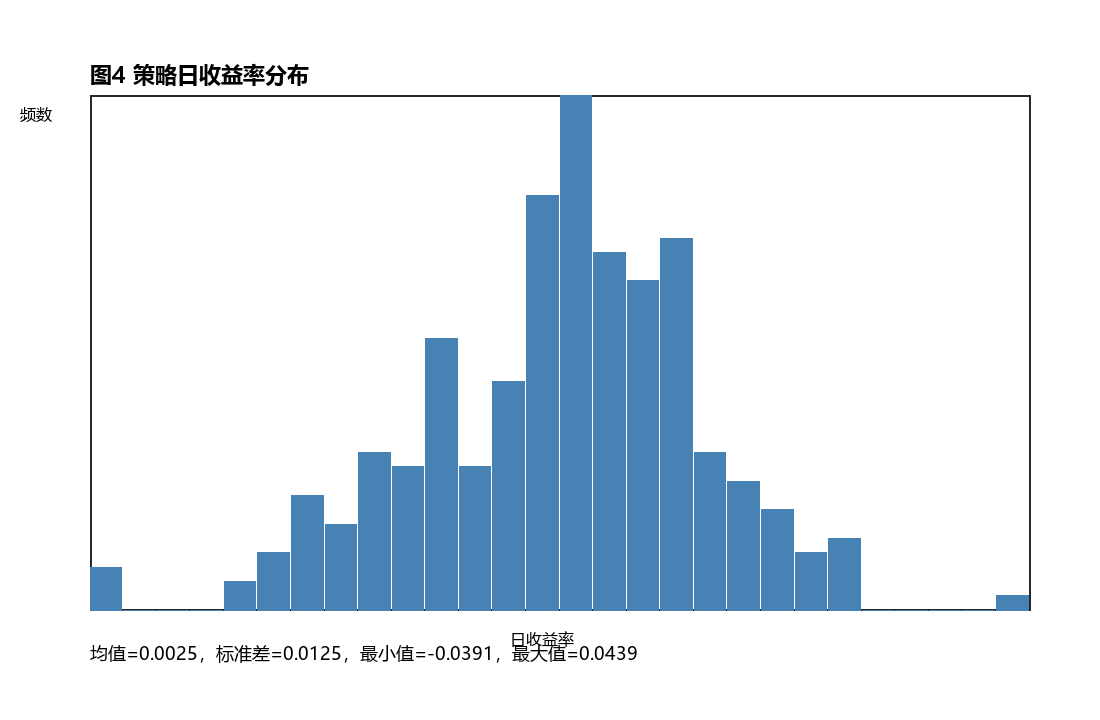
\includegraphics[width=0.86\textwidth]{return_distribution.png}
\caption{策略日收益率分布}
\label{fig:hist}
\end{figure}

\subsection{模型设定}
本文采用逐步扩展的多元线性回归模型。模型(1)只控制上证指数收益，用于观察策略与最基础市场基准之间的关系：
\begin{equation}
R_{p,t}=\alpha+\beta_1R_{SH,t}+\varepsilon_t .
\end{equation}
模型(2)加入深证成指和中证500收益，用于识别策略是否同时受不同市场板块影响：
\begin{equation}
R_{p,t}=\alpha+\beta_1R_{SH,t}+\beta_2R_{SZ,t}+\beta_3R_{ZZ500,t}+\varepsilon_t .
\end{equation}
模型(3)加入换手率，用于检验调仓强度是否与当日收益相关：
\begin{equation}
R_{p,t}=\alpha+\beta_1R_{SH,t}+\beta_2R_{SZ,t}+\beta_3R_{ZZ500,t}+\gamma Turnover_t+\varepsilon_t .
\end{equation}
模型(4)进一步加入成本率，作为交易摩擦控制变量：
\begin{equation}
R_{p,t}=\alpha+\beta_1R_{SH,t}+\beta_2R_{SZ,t}+\beta_3R_{ZZ500,t}+\gamma Turnover_t+\delta Cost_t+\varepsilon_t .
\end{equation}

上述模型均使用OLS估计。将被解释变量写成向量$Y$，解释变量矩阵写成$X$，则普通最小二乘估计量为
\begin{equation}
\hat{\beta}=(X'X)^{-1}X'Y.
\end{equation}
残差向量为
\begin{equation}
\hat{\varepsilon}=Y-X\hat{\beta}.
\end{equation}
考虑到金融收益率序列常见异方差，本文在回归表中报告HC3稳健标准误。White提出的异方差稳健协方差矩阵为后续稳健推断提供了基础\cite{white1980}，MacKinnon和White进一步讨论了HC系列修正形式\cite{mackinnon1985}。HC3协方差矩阵可表示为
\begin{equation}
\widehat{Var}_{HC3}(\hat{\beta})=(X'X)^{-1}X'\hat{\Omega}_{HC3}X(X'X)^{-1},
\end{equation}
其中$\hat{\Omega}_{HC3}$为对角矩阵，其第$t$个对角元素为
\begin{equation}
\frac{\hat{\varepsilon}_t^2}{(1-h_{tt})^2},
\end{equation}
$h_{tt}$为帽子矩阵$H=X(X'X)^{-1}X'$的第$t$个对角元素。HC3稳健标准误对高杠杆观测更敏感，适合样本量中等且可能存在异常波动的日频收益数据。模型解释的重点不是追求最高$R^2$，而是判断市场变量和交易变量是否显著，以及控制这些变量后策略是否仍存在统计意义上的异常收益。

在模型设定上，本文采取从简单到复杂的递进方式，而不是一次性放入所有变量。这样做有两个好处。第一，可以观察核心市场变量进入模型后，系数、显著性和拟合优度如何变化。例如，若模型(1)中的上证指数系数很高，而加入中证500后上证指数系数下降，就说明原先由上证指数吸收的一部分解释力实际上来自其他市场板块。第二，可以避免直接给出复杂模型而缺少解释过程。回归分析课程强调模型设定的可解释性，逐步扩展模型能够更清楚地展示研究者如何从单指数模型过渡到多变量控制模型。

此外，本文没有把LightGBM预测分数直接作为解释变量放入主回归。原因是预测分数本身由大量Alpha158特征训练得到，属于模型输出变量，直接放入回归可能造成解释层次混乱。本文更关注策略实现后的收益序列是否受到市场和交易行为影响，因此主回归以组合收益率为被解释对象。若后续进行深入研究，可以另设一个横截面回归问题：用个股未来收益回归预测分数和控制变量，以检验预测分数在个股层面的解释力。本文限于课程论文篇幅，将重点放在时间序列层面的策略收益解释。

\section{实证检验}
\subsection{数据来源和描述性分析}
本文所有行情数据均来自新浪财经公开页面及其行情接口\cite{sinafinance}。股票列表通过新浪市场中心分页接口获取，日K线通过新浪历史K线接口获取，复权因子通过新浪复权因子接口获取，指数数据包括上证指数、深证成指、上证100、深证100和中证500。数据处理流程包括接口探测、股票池过滤、日K线抓取、复权因子解析、标准CSV生成、Qlib CSV生成、Qlib二进制数据dump、模型训练和回测分析。项目最终覆盖5206只A股股票，标准日频样本超过636万行。由于新浪历史K线不返回历史成交额，本文没有编造amount和vwap字段。

更具体地说，接口探测阶段发现新浪历史K线日频参数为$scale=240$，当前可稳定请求的最大$datalen$约为1970；历史K线返回字段包括日期、开盘价、最高价、最低价、收盘价和成交量，但不返回历史成交额。股票池构造阶段优先使用手工股票池文件，若不存在则分页请求新浪市场中心节点，包括沪市A股、深市A股、创业板和科创板，并过滤北交所等不属于本文研究范围的标的。复权因子阶段优先使用后复权因子，若后复权失败才考虑前复权，若均失败则将该股票标记为$factor=1$的fallback样本。

Qlib转换阶段使用如下归一化思想。设原始未复权收盘价为$C_{i,t}$，新浪复权因子为$F_{i,t}$，样本起点的复权收盘价为$C_{i,0}F_{i,0}$，则Qlib中用于特征计算的归一化收盘价可写为
\begin{equation}
\tilde{C}_{i,t}=\frac{C_{i,t}F_{i,t}}{C_{i,0}F_{i,0}}.
\end{equation}
开盘价、最高价和最低价采用相同方式归一化。对应的Qlib factor可写为
\begin{equation}
\tilde{F}_{i,t}=\frac{F_{i,t}}{C_{i,0}F_{i,0}},
\end{equation}
成交量则按Qlib约定使用调整后的factor进行反向处理。该处理保证了价格序列在复权意义上连续，也使Alpha158特征能够在统一尺度下计算。

在建模流程上，训练期为2021年1月4日至2024年4月16日，验证期为2024年4月17日至2025年5月22日，测试期为2025年5月23日至2026年6月25日。训练期和测试期没有日期重叠。模型使用Alpha158特征，标签为未来收益，标签用于监督学习是正常做法。Qlib Alpha158默认标签可表示为
\begin{equation}
LABEL_{i,t}=\frac{Ref(C_{i,t},-2)}{Ref(C_{i,t},-1)}-1,
\end{equation}
即用未来一期收益作为训练目标。关键在于标签不能泄露进特征，也不能在回测成交时点形成未来函数。本文采用上一交易日信号在下一交易日开盘成交，避免使用当天收盘后才能得到的特征按当天收盘成交。这个处理使回测更接近可执行交易逻辑。

图\ref{fig:nav}展示策略与五个基准的净值对比。可以看到，策略测试期净值增长较快，但并非单调上升，中间存在明显回撤。图\ref{fig:drawdown}进一步展示回撤过程，说明策略虽然收益较高，但仍然会经历较大短期损失。对于回归分析而言，这两张图的作用不是直接证明策略有效，而是帮助理解被解释变量的时间序列特征。

从数据质量角度看，本文对项目数据作了两项特别处理。第一，历史K线中没有成交额字段，因此标准数据中的amount和vwap保留为空值，不用实时成交额倒填历史成交额，也不用成交量和价格近似编造成交额。这样虽然减少了可用变量，但避免了人为制造数据。第二，复权因子只允许向前填充，不允许用未来日期的因子向过去回填。复权因子会影响Qlib中的复权价格和Alpha158特征，如果处理不当，可能造成未来信息泄露。本文在最终版本中去除了向后回填逻辑，使特征构造更符合历史可得信息原则。

在交易设定方面，本文最终采用开盘成交而非收盘成交。原因在于，Alpha158特征通常包含当日收盘价、成交量等信息，这些信息只有收盘后才完整可得。虽然Qlib策略本身会使用上一交易日信号生成当前交易日决策，但若成交价格设置为收盘价，仍然偏向理想化。改为下一交易日开盘价成交后，策略收益从原先更高的水平下降到当前结果，说明成交假设对回测结论有实质影响。这一过程也体现了实证研究中的审慎原则：当发现假设可能过于乐观时，应主动采用更保守的设定。

\begin{figure}[H]
\centering
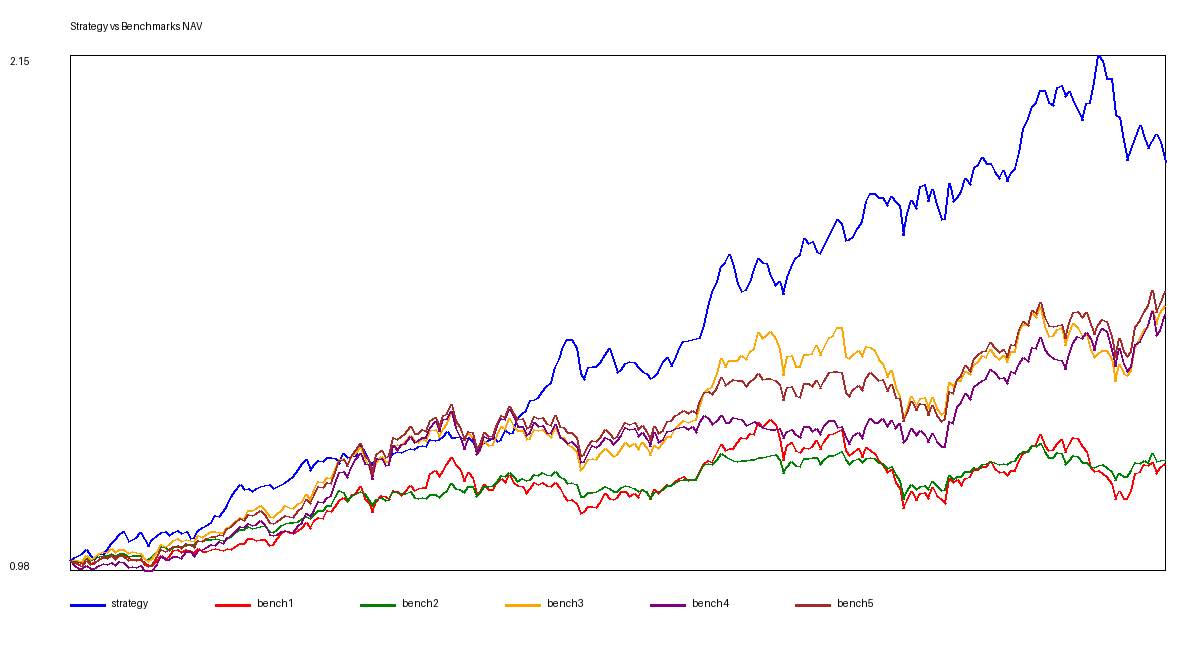
\includegraphics[width=0.92\textwidth]{nav_compare_all.png}
\caption{策略与五个基准指数的净值对比}
\label{fig:nav}
\end{figure}

\begin{figure}[H]
\centering
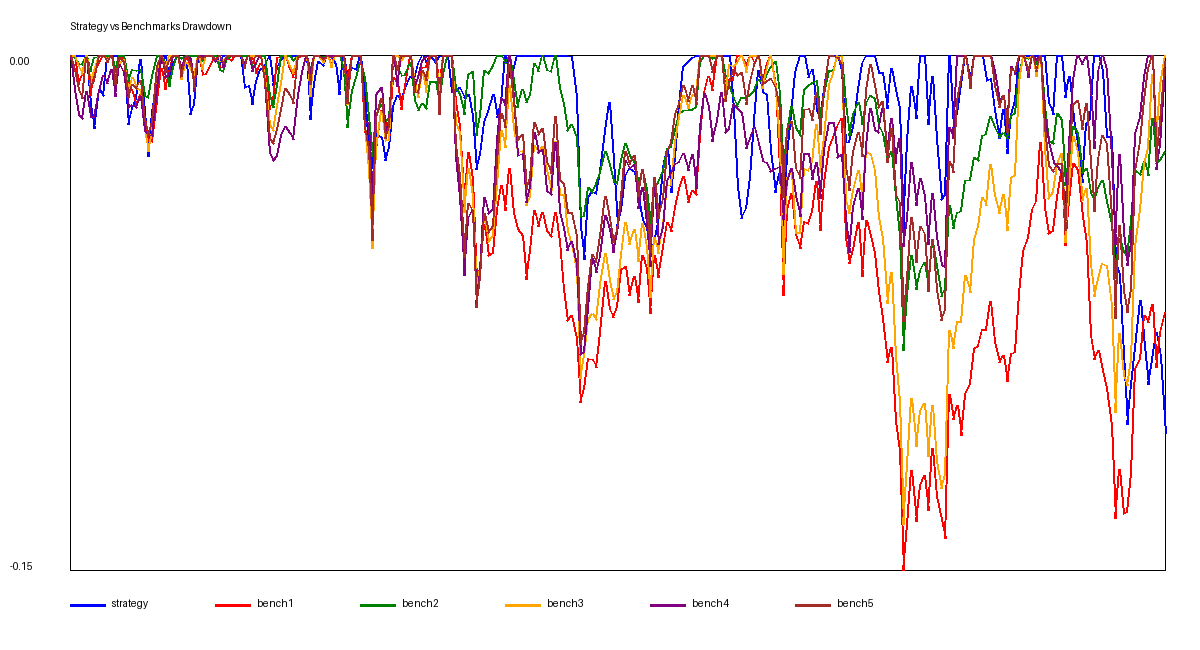
\includegraphics[width=0.92\textwidth]{drawdown_compare_all.png}
\caption{策略与五个基准指数的回撤对比}
\label{fig:drawdown}
\end{figure}

\subsection{相关检验}
在多元回归中，如果解释变量之间高度相关，会导致系数估计不稳定、标准误变大，从而影响显著性判断。本文首先绘制主要变量相关系数热力图，如图\ref{fig:heatmap}所示。市场指数之间存在较明显正相关，这符合A股市场不同指数同涨同跌的现实特征；策略收益与主要指数也存在正相关，说明策略并非完全市场中性。换手率与收益之间的相关性较弱，说明单纯高换手并不必然带来更高收益。

\begin{figure}[H]
\centering
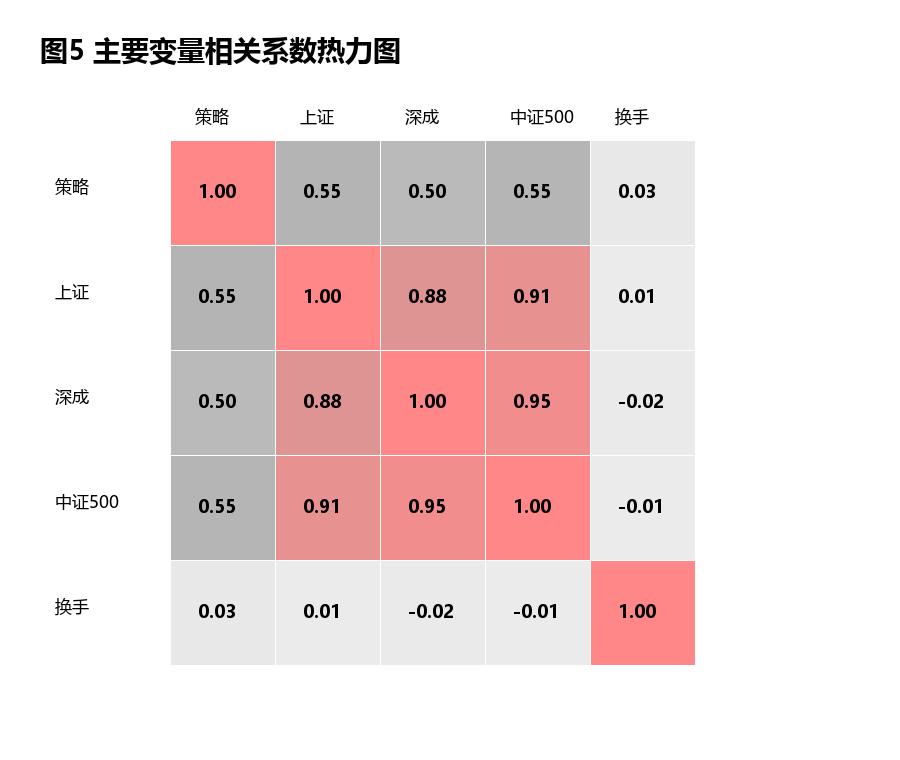
\includegraphics[width=0.78\textwidth]{correlation_heatmap.png}
\caption{主要变量相关系数热力图}
\label{fig:heatmap}
\end{figure}

图\ref{fig:scatter}给出了策略收益与上证指数收益的散点图。散点整体呈正斜率，说明市场上涨日策略通常也更容易取得正收益；但散点离回归线仍有明显分散，说明策略收益并不能完全由上证指数解释。图\ref{fig:rolling}展示60日滚动beta和滚动相关系数，可以看到市场暴露并非固定不变，而是随行情阶段变化。这也提示我们，单一全样本回归只能给出平均关系，后续研究可进一步采用滚动回归或分阶段回归。

\begin{figure}[H]
\centering
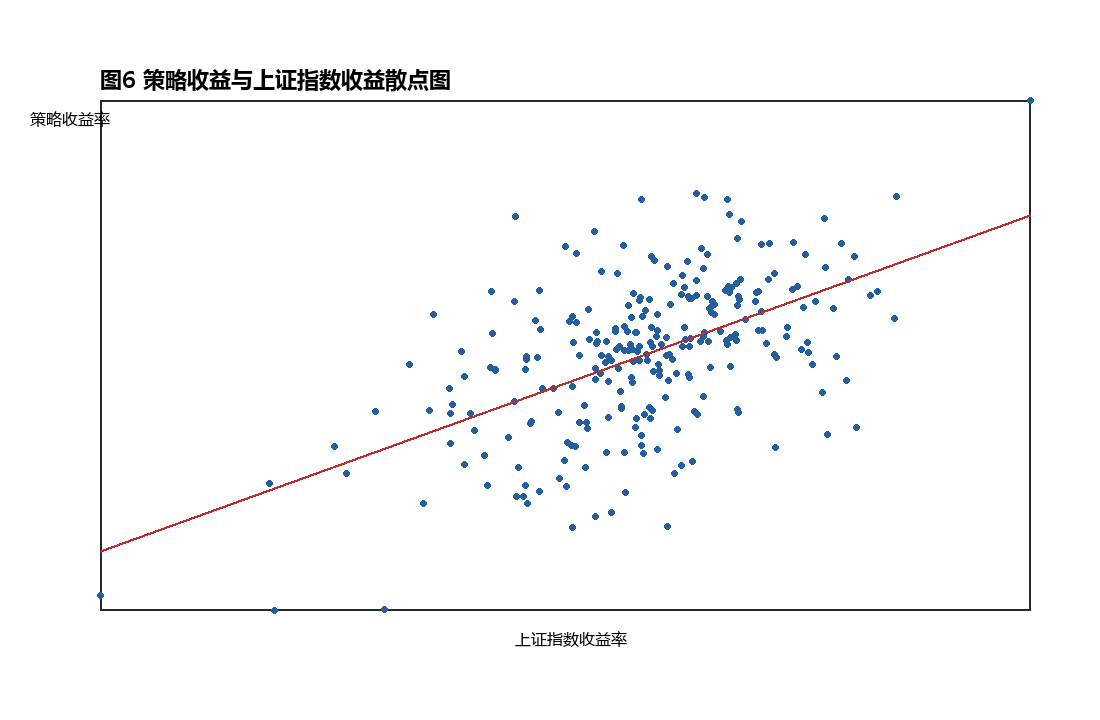
\includegraphics[width=0.86\textwidth]{scatter_strategy_sh.png}
\caption{策略收益与上证指数收益散点图}
\label{fig:scatter}
\end{figure}

\begin{figure}[H]
\centering
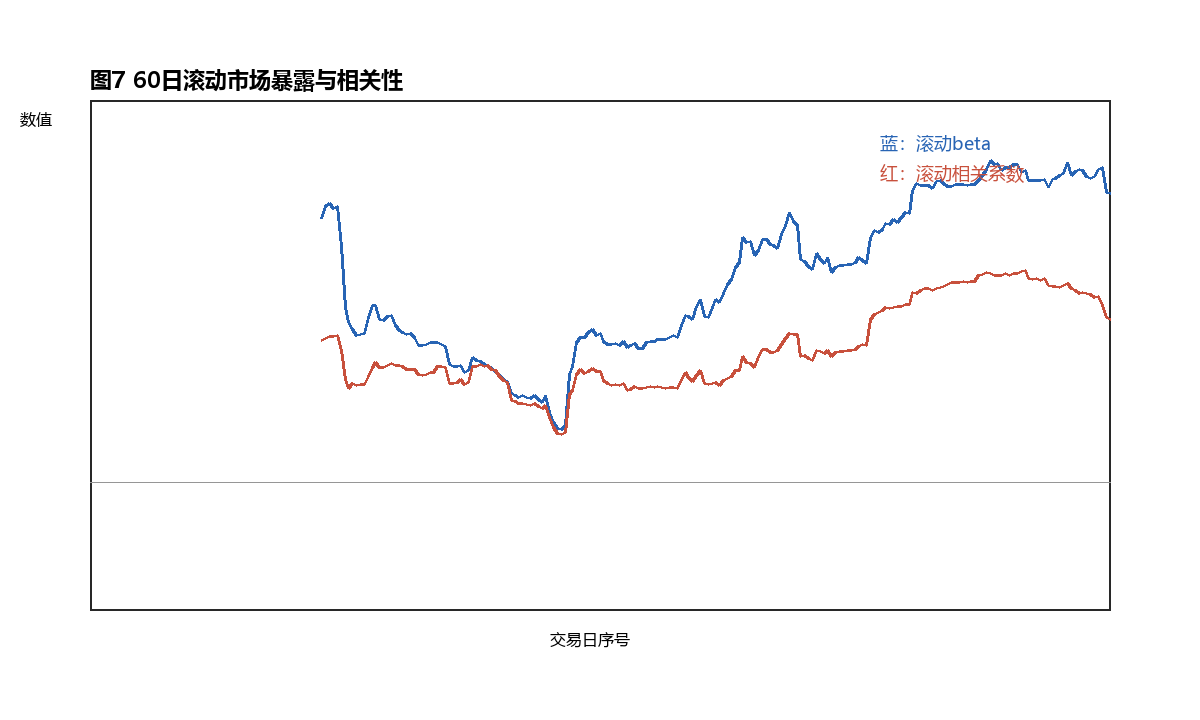
\includegraphics[width=0.92\textwidth]{rolling_beta_corr.png}
\caption{60日滚动市场暴露与相关性}
\label{fig:rolling}
\end{figure}

表\ref{tab:diag}报告模型诊断结果。Durbin-Watson统计量用于判断残差一阶自相关\cite{durbin1951}，其形式为
\begin{equation}
DW=\frac{\sum_{t=2}^{T}(\hat{\varepsilon}_t-\hat{\varepsilon}_{t-1})^2}{\sum_{t=1}^{T}\hat{\varepsilon}_t^2}.
\end{equation}
Breusch-Pagan检验用于判断异方差\cite{breusch1979}，其基本思想是用残差平方对解释变量作辅助回归，若辅助回归解释力较强，则说明误差方差可能与解释变量有关。其LM统计量可写为
\begin{equation}
LM=T R_{aux}^2.
\end{equation}
VIF用于衡量解释变量之间的共线性。对第$j$个解释变量，若用其他解释变量回归该变量得到$R_j^2$，则
\begin{equation}
VIF_j=\frac{1}{1-R_j^2}.
\end{equation}
Jarque-Bera检验用于判断残差是否接近正态分布\cite{jarque1980}，统计量为
\begin{equation}
JB=\frac{T}{6}\left(S^2+\frac{(K-3)^2}{4}\right),
\end{equation}
其中$S$为偏度，$K$为峰度。诊断结果显示，金融收益率数据并不完全满足经典线性回归的理想条件，因此本文使用稳健标准误是必要的。同时，最大VIF较高，说明市场指数之间确实存在共线性，解释单个市场系数时需要谨慎，更应关注模型整体解释力和符号方向。

\begin{table}[H]
\centering
\caption{模型诊断检验结果}
\label{tab:diag}
\begin{tabular}{lrl}
\toprule
诊断指标 & 数值 & 说明 \\
\midrule
Durbin-Watson统计量 & 1.4829 & 接近2表示一阶自相关较弱 \\
Breusch-Pagan LM & 5.5408 & 异方差检验统计量 \\
BP检验p值 & 0.3535 & p值较小说明异方差风险较强 \\
Jarque-Bera统计量 & 2.2239 & 残差正态性检验统计量 \\
JB检验p值 & 0.3289 & p值较小说明残差偏离正态 \\
最大VIF & 13.1703 & 衡量解释变量共线性 \\
\bottomrule
\end{tabular}
\end{table}

\begin{figure}[H]
\centering
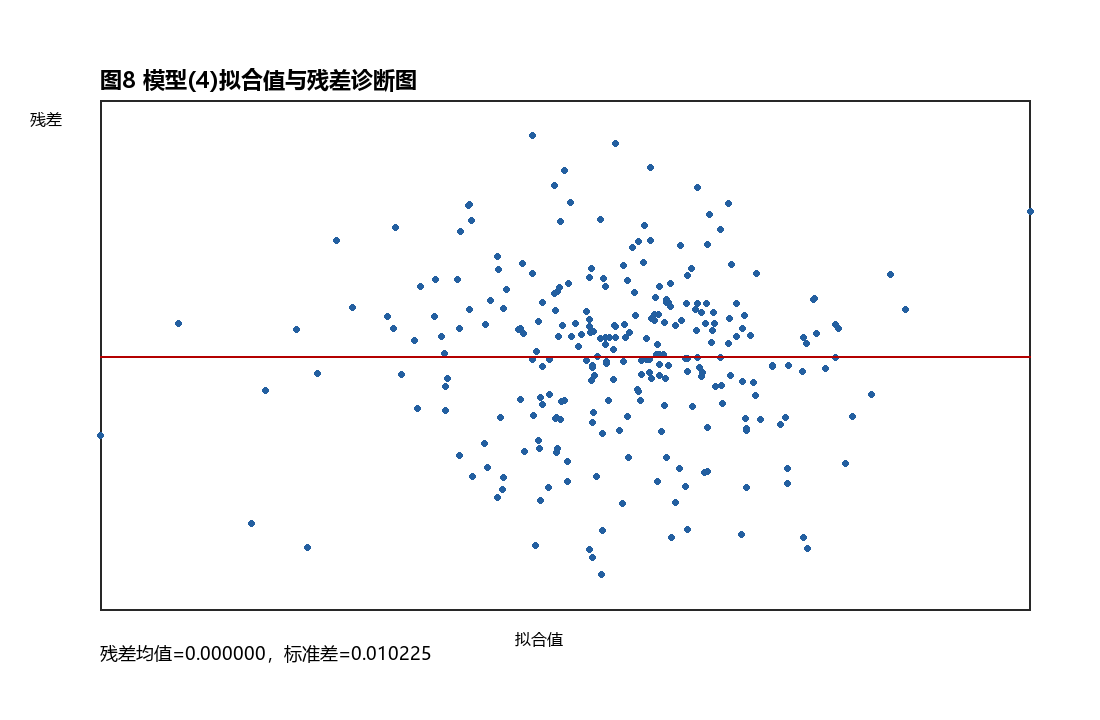
\includegraphics[width=0.86\textwidth]{regression_residuals.png}
\caption{模型(4)拟合值与残差关系}
\label{fig:resid}
\end{figure}

\subsection{实证回归结果及分析}
表\ref{tab:reg}报告四个模型的回归结果。模型(1)显示，上证指数收益系数显著为正，说明策略收益与市场整体行情存在明显关系。换言之，策略收益并不是完全独立于市场的绝对收益。模型(2)加入深证成指和中证500后，模型解释力提高，其中中证500收益系数显著为正，说明策略收益与中小市值股票行情具有较强关联。这一结果与全A选股和TopK持仓方式相符，因为模型可能更容易在中小市值股票中获得较高弹性。

模型(3)加入换手率后，换手率系数并不显著。这说明在当前样本中，调仓强度本身不能稳定解释策略当日收益。模型(4)进一步加入成本率，成本率变量的解释力同样有限，可能原因是成本率与换手率高度相关，而且当前成本设定仍然是模型化交易成本，尚未包含真实盘口冲击成本。因此，不能简单认为提高换手就能提高收益，也不能认为当前回测成本已经完全反映实盘摩擦。

\begin{table}[H]
\centering
\caption{策略日收益率的OLS回归结果}
\label{tab:reg}
\begin{threeparttable}
\begin{tabular}{lcccc}
\toprule
变量 & 模型(1) & 模型(2) & 模型(3) & 模型(4) \\
\midrule
常数项 & 0.0018*** & 0.0018*** & 0.0002 & -0.0018 \\
 & (0.0007) & (0.0006) & (0.0024) & (0.0054) \\
上证指数收益 & 0.8647*** & 0.5388*** & 0.5347*** & 0.5282*** \\
 & (0.0886) & (0.1927) & (0.1916) & (0.1902) \\
深证成指收益 &  & -0.2665* & -0.2636* & -0.2649* \\
 &  & (0.1599) & (0.1601) & (0.1605) \\
中证500收益 &  & 0.4630*** & 0.4627*** & 0.4680*** \\
 &  & (0.1672) & (0.1675) & (0.1679) \\
换手率 &  &  & 0.0071 & -0.0056 \\
 &  &  & (0.0097) & (0.0331) \\
成本率 &  &  &  & 21.9613 \\
 &  &  &  & (47.6697) \\
\midrule
样本量 & 265 & 265 & 265 & 265 \\
$R^2$ & 0.3048 & 0.3249 & 0.3257 & 0.3265 \\
调整$R^2$ & 0.3021 & 0.3171 & 0.3153 & 0.3135 \\
\bottomrule
\end{tabular}
\begin{tablenotes}
\small
\item 注：括号内为HC3稳健标准误；***、**、*分别表示在1\%、5\%、10\%水平上显著。
\end{tablenotes}
\end{threeparttable}
\end{table}

从经济含义看，市场指数收益系数显著为正意味着策略承担了权益市场方向性风险。若投资者只看策略总收益，可能会误以为收益完全来自模型选股能力；但回归结果表明，其中一部分收益可由市场上涨和中小盘行情解释。常数项在部分模型中为正，说明控制市场因素后策略仍可能存在一定异常收益，但这一结论必须谨慎。原因在于本文仍使用当前时点股票池，不能完全排除幸存者偏差；复权因子和股票列表也不是严格历史时点数据库；此外，真实交易中还可能面临更高滑点、成交量约束和涨跌停无法成交等问题。

表\ref{tab:perf}展示策略相对于五个基准的表现。策略收益高于各基准，但相对于中证500和深证成指的超额收益明显低于相对于上证指数的超额收益。这与回归结果相互印证：策略更接近权益市场中高弹性板块，而不是完全独立于市场。若未来进一步完善研究，可以将行业收益、规模因子、估值因子和动量因子纳入模型，以检验常数项是否仍然显著。

\begin{table}[H]
\centering
\caption{策略与五个基准的收益表现}
\label{tab:perf}
\begin{tabular}{llrrrr}
\toprule
基准 & 代码 & 策略收益 & 基准收益 & 超额收益 & 最大回撤 \\
\midrule
上证指数 & sh000001 & 0.9058 & 0.2305 & 0.6752 & -0.1134 \\
上证100 & sh000132 & 0.9058 & 0.2206 & 0.6851 & -0.1134 \\
中证500 & sh000905 & 0.9058 & 0.5811 & 0.3247 & -0.1134 \\
深证成指 & sz399001 & 0.9058 & 0.6130 & 0.2927 & -0.1134 \\
深证100 & sz399330 & 0.9058 & 0.5602 & 0.3456 & -0.1134 \\
\bottomrule
\end{tabular}
\end{table}

\subsection{稳健性与回测可信度讨论}
本文在项目实现过程中对回测可信度进行了专门检查。首先，训练期、验证期和测试期在日期上没有重叠，模型没有直接在测试期拟合参数。其次，Alpha158标签使用未来收益，这是监督学习中构造训练目标的正常方式，关键在于标签不能泄露到测试特征中。再次，Qlib的TopkDropoutStrategy在生成交易决策时使用上一交易日预测信号，本文又将成交价格改为下一交易日开盘价，因此避免了“当天收盘后才知道的信息按当天收盘成交”的明显时间穿越。

但是，本文仍然承认回测存在局限。第一，股票池来自当前新浪可获取股票列表，不是严格历史成分股池，可能排除了已经退市或长期不可交易股票，从而形成幸存者偏差。第二，新浪公开接口不提供完整历史成交额和盘口深度，本文无法精确估计冲击成本。第三，回测中的涨跌停、停牌和成交约束虽然有一定处理，但仍难以完全模拟真实交易。第四，测试期只有265个交易日，样本长度有限，若市场环境变化，回归系数和策略表现可能发生变化。

因此，本文对结果采取审慎解释：策略在测试期表现较好，说明模型可能捕捉到一定横截面排序信息；回归结果显示策略收益与市场变量显著相关，说明收益并非完全独立；诊断检验提示经典线性回归假设并不完全满足，说明需要稳健标准误和进一步稳健性分析。这样的结论比单纯声称“策略收益很高”更加符合回归分析课程论文的要求。

还需要指出的是，回归分析并不能替代所有金融风险检验。OLS模型揭示的是平均线性关系，而真实策略风险还包括尾部风险、流动性风险、模型失效风险和参数不稳定风险。例如，在市场快速下跌或流动性突然收缩时，开盘价成交假设可能仍然过于理想；在股票涨跌停或停牌时，策略计划中的调仓也可能无法完成。因此，本文将回归结果作为解释工具，而不是作为交易决策的唯一依据。对课程论文而言，这种边界意识同样重要，因为它说明研究者理解模型适用范围，没有把统计显著性机械等同于经济可行性。

如果把本文结果与常见课程案例相比，本研究的数据更贴近真实市场，变量之间的关系也更加复杂。许多教材案例中的解释变量相对独立，误差项也较容易满足经典假设；而金融日频数据往往同时存在高相关、异方差、异常值和非平稳等问题。正因为如此，本文没有只给出一张回归表，而是配合净值图、回撤图、收益分布图、相关热力图、散点图、滚动beta图和残差图共同解释。多图并用的目的不是装饰论文，而是帮助读者从不同角度理解同一个回归问题。

\section{结论及对策建议}
本文基于新浪财经公开数据构建了一个A股量化研究项目，并在此基础上完成回归分析。项目层面，本文实现了从公开接口抓取数据、标准化清洗、Qlib格式转换、Alpha158-LightGBM训练预测到策略回测的完整流程。论文层面，本文没有停留在工程复现，而是将策略测试期收益作为被解释变量，构建多元线性回归模型，分析其与市场指数收益、换手率和成本率之间的关系。

实证结果表明，在较保守的下一交易日开盘成交设定下，策略测试期仍取得高于主要基准的收益；但回归结果也表明，策略收益显著暴露于上证指数和中证500等市场变量，说明收益并非完全来自个股选择能力。模型诊断进一步显示，金融日频收益数据存在共线性和异方差风险，因此在解释回归系数时必须使用稳健标准误，并避免对单个系数作过度解释。

本文的主要结论可以概括为三点。第一，机器学习量化策略的净值结果必须经过回归分解，才能判断收益来源。第二，市场指数收益对策略收益具有显著解释力，说明策略不是市场中性策略。第三，当前回测结果具有研究价值，但仍受到公开数据源、当前股票池和交易成本假设的限制，不能直接等同于实盘收益。

基于上述结论，本文提出以下建议。第一，后续研究应构建point-in-time股票池，纳入历史退市、停牌和上市时间信息，以减少幸存者偏差。第二，应进一步加入行业、规模、估值、动量和波动率等控制变量，建立更完整的多因子回归模型。第三，应采用更严格的交易成本和滑点假设，尤其对于高换手策略，需要加入成交量约束和冲击成本。第四，应进行滚动窗口回归和分市场阶段回归，检验模型系数是否稳定。第五，应将机器学习预测分数本身也纳入回归框架，检验预测分数对未来收益是否具有增量解释力。

总之，本文把一个A股量化项目转化为回归分析课程论文，重点不在于夸大策略收益，而在于展示如何用回归方法解释、检验和约束量化回测结果。通过这种处理，量化项目不再只是工程实践，而成为一个包含变量设定、模型估计、统计检验和经济解释的完整实证研究。

本文也为后续课程学习提供了一个启示：回归分析并不局限于传统宏观经济或企业财务数据，只要研究者能够明确被解释变量和解释变量，并能说明变量之间的经济逻辑，就可以将回归方法应用到更复杂的数据场景中。量化投资项目往往看起来属于计算机或金融工程任务，但其最终结果仍然需要统计检验来回答“收益从何而来”这一问题。正是在这个意义上，本文把工程项目、金融市场和回归分析三个部分连接起来，使期末论文既有实际项目支撑，又能体现课程方法训练。

\addcontentsline{toc}{section}{参考文献}
\begin{thebibliography}{99}
\bibitem{sharpe1964} Sharpe W F. Capital asset prices: A theory of market equilibrium under conditions of risk[J]. The Journal of Finance, 1964, 19(3): 425--442.
\bibitem{fama1993} Fama E F, French K R. Common risk factors in the returns on stocks and bonds[J]. Journal of Financial Economics, 1993, 33(1): 3--56.
\bibitem{fama2015} Fama E F, French K R. A five-factor asset pricing model[J]. Journal of Financial Economics, 2015, 116(1): 1--22.
\bibitem{jegadeesh1993} Jegadeesh N, Titman S. Returns to buying winners and selling losers: Implications for stock market efficiency[J]. The Journal of Finance, 1993, 48(1): 65--91.
\bibitem{carhart1997} Carhart M M. On persistence in mutual fund performance[J]. The Journal of Finance, 1997, 52(1): 57--82.
\bibitem{gu2020} Gu S, Kelly B, Xiu D. Empirical asset pricing via machine learning[J]. The Review of Financial Studies, 2020, 33(5): 2223--2273.
\bibitem{ke2017} Ke G, Meng Q, Finley T, et al. LightGBM: A highly efficient gradient boosting decision tree[C]//Advances in Neural Information Processing Systems. 2017, 30.
\bibitem{yang2020} Yang X, Liu W, Zhou D, et al. Qlib: An AI-oriented quantitative investment platform[EB/OL]. arXiv preprint arXiv:2009.11189, 2020.
\bibitem{qlibgithub} Microsoft. Qlib: An AI-oriented quantitative investment platform[EB/OL]. GitHub repository, \url{https://github.com/microsoft/qlib}, accessed 2026-06-29.
\bibitem{sinafinance} 新浪财经. 新浪财经股票行情中心[EB/OL]. \url{https://finance.sina.com.cn/stock/}, accessed 2026-06-29.
\bibitem{white1980} White H. A heteroskedasticity-consistent covariance matrix estimator and a direct test for heteroskedasticity[J]. Econometrica, 1980, 48(4): 817--838.
\bibitem{mackinnon1985} MacKinnon J G, White H. Some heteroskedasticity-consistent covariance matrix estimators with improved finite sample properties[J]. Journal of Econometrics, 1985, 29(3): 305--325.
\bibitem{breusch1979} Breusch T S, Pagan A R. A simple test for heteroscedasticity and random coefficient variation[J]. Econometrica, 1979, 47(5): 1287--1294.
\bibitem{durbin1951} Durbin J, Watson G S. Testing for serial correlation in least squares regression. II[J]. Biometrika, 1951, 38(1/2): 159--178.
\bibitem{jarque1980} Jarque C M, Bera A K. Efficient tests for normality, homoscedasticity and serial independence of regression residuals[J]. Economics Letters, 1980, 6(3): 255--259.
\end{thebibliography}

\end{document}
